\documentclass[border=10pt]{standalone}
\usepackage{tikz}
\usetikzlibrary{arrows.meta, positioning, shapes.geometric, fit, backgrounds}

\definecolor{layer1}{HTML}{E8D5F5}
\definecolor{layer2}{HTML}{D5E8F5}
\definecolor{layer3}{HTML}{D5F5E0}
\definecolor{layer4}{HTML}{F5ECD5}
\definecolor{layer5}{HTML}{F5D5D5}
\definecolor{layer6}{HTML}{F0F0F0}

\begin{document}
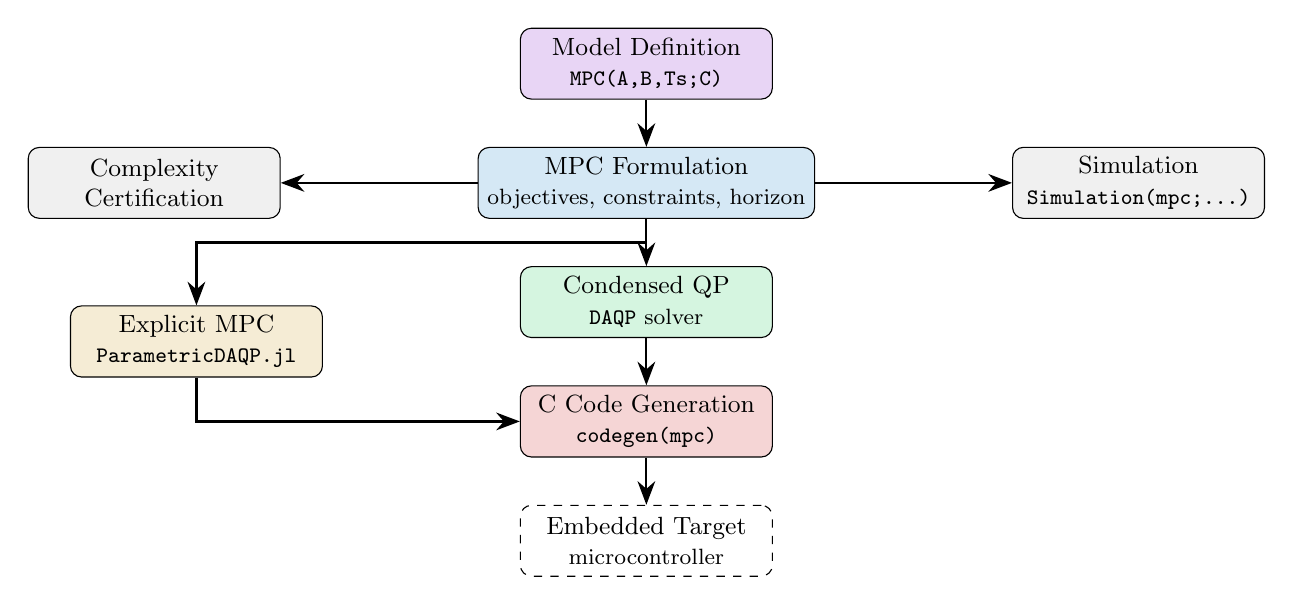
\begin{tikzpicture}[
    node distance=0.6cm and 0.8cm,
    block/.style={rectangle, draw, rounded corners, minimum width=3.2cm, minimum height=0.9cm, align=center, font=\small},
    arrow/.style={-{Stealth[length=3mm]}, thick},
    label/.style={font=\footnotesize\itshape, text=gray},
]

% Model layer
\node[block, fill=layer1] (model) {Model Definition\\{\footnotesize\texttt{MPC(A,B,Ts;C)}}};

% MPC formulation
\node[block, fill=layer2, below=of model] (formulation) {MPC Formulation\\{\footnotesize objectives, constraints, horizon}};

% Simulation branch
\node[block, fill=layer6, right=2.5cm of formulation] (sim) {Simulation\\{\footnotesize\texttt{Simulation(mpc;...)}}};

% Optimization
\node[block, fill=layer3, below=of formulation] (qp) {Condensed QP\\{\footnotesize \texttt{DAQP} solver}};

% Explicit MPC branch
\node[block, fill=layer4, left=2.5cm of qp, yshift=-0.5cm] (explicit) {Explicit MPC\\{\footnotesize \texttt{ParametricDAQP.jl}}};

% Certification branch
\node[block, fill=layer6, left=2.5cm of formulation] (cert) {Complexity\\Certification};

% Code generation
\node[block, fill=layer5, below=of qp] (codegen) {C Code Generation\\{\footnotesize\texttt{codegen(mpc)}}};

% Embedded target
\node[block, fill=white, draw, dashed, below=of codegen] (embedded) {Embedded Target\\{\footnotesize microcontroller}};

% Arrows
\draw[arrow] (model) -- (formulation);
\draw[arrow] (formulation) -- (qp);
\draw[arrow] (qp) -- (codegen);
\draw[arrow] (codegen) -- (embedded);
\draw[arrow] (formulation) -- (sim);
\draw[arrow] (formulation) -- (cert);
\draw[arrow] (formulation.south) -- ++(0,-0.3) -| (explicit.north);
\draw[arrow] (explicit.south) |- (codegen.west);

\end{tikzpicture}
\end{document}
